\section{Evaluation}
\label{sec:evaluation}

\begin{figure}[t]
    \centering
    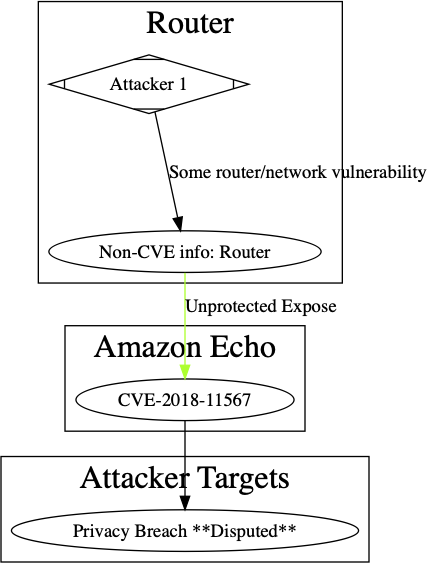
\includegraphics[width=0.20\textwidth]{exploitability_circuit1cve.png}
    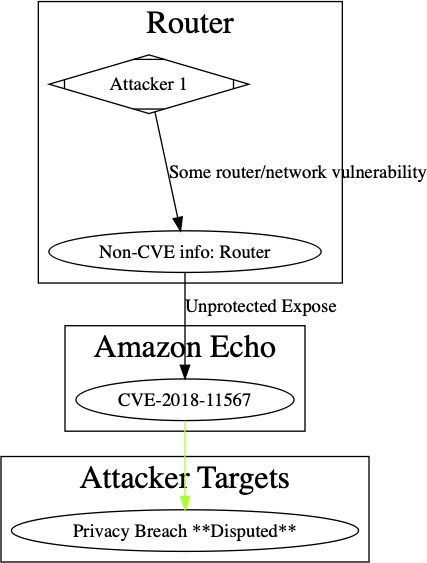
\includegraphics[width=0.20\textwidth]{impact_circuit1cve.png}
    \caption{Exploitability (left) and impact (right) circuits corresponding to one device under the observation of a single vulnerability.}
    \label{fig:exp1cve}
\end{figure}

\begin{figure}[t]
    \centering
    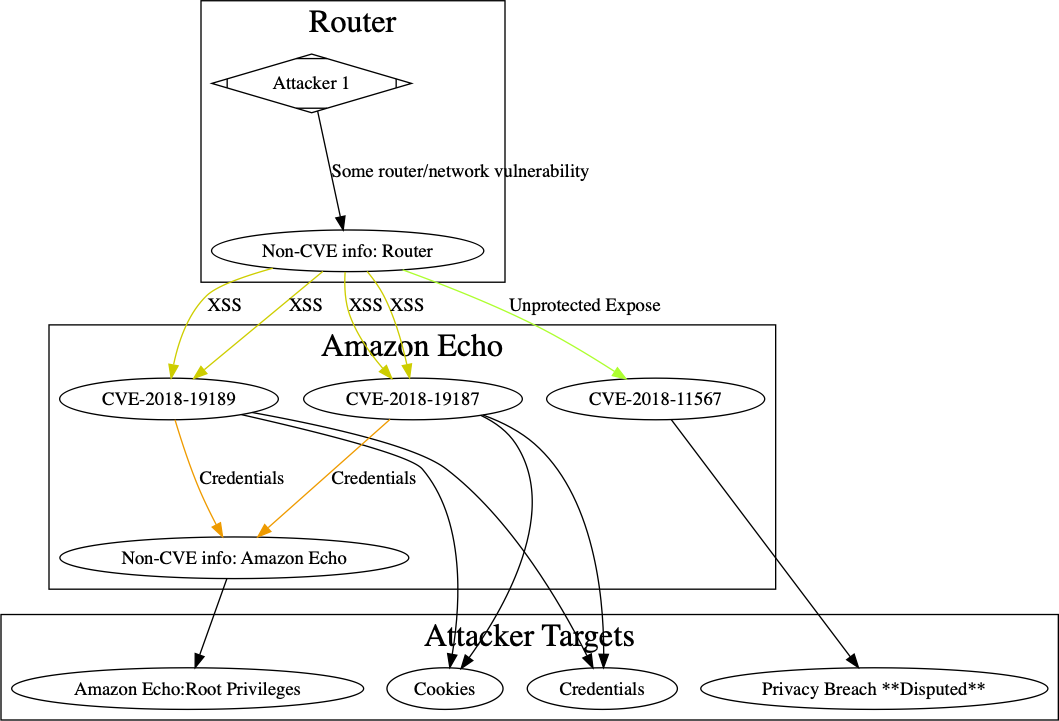
\includegraphics[width=0.40\textwidth]{exploitability_circuit1dev.png}
    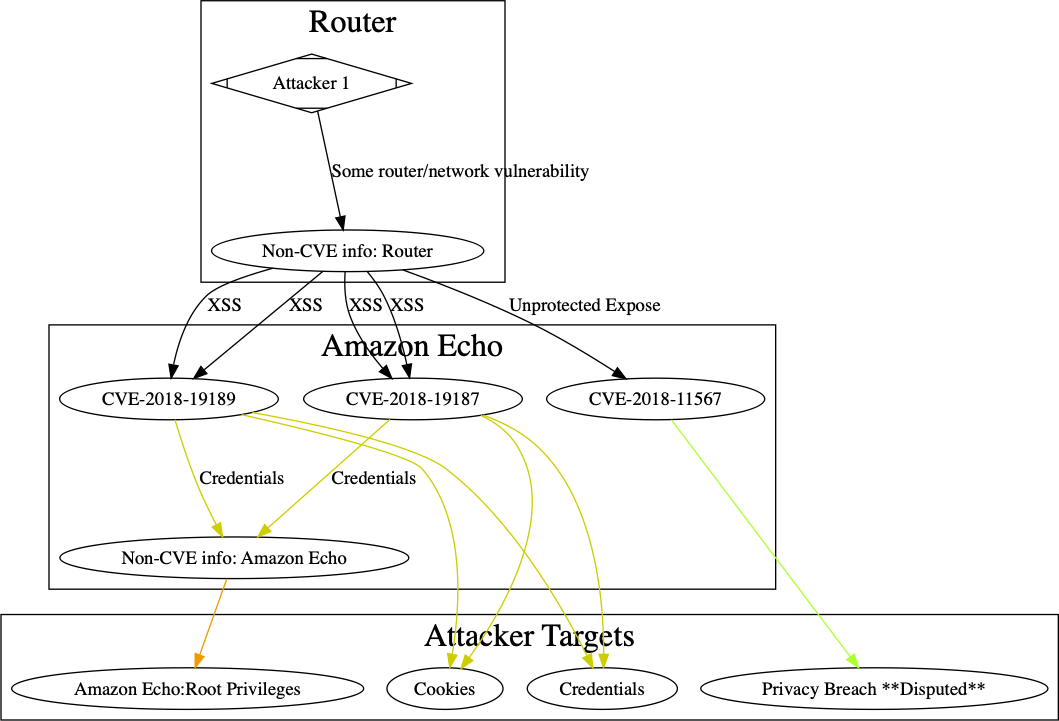
\includegraphics[width=0.40\textwidth]{impact_circuit1dev.png}
    \caption{Exploitability (top) and impact (bottom) circuits corresponding to one device under the observation of all vulnerabilities.}
    \label{fig:exp1dev}
\end{figure}

\begin{figure*}[t]
    \centering
    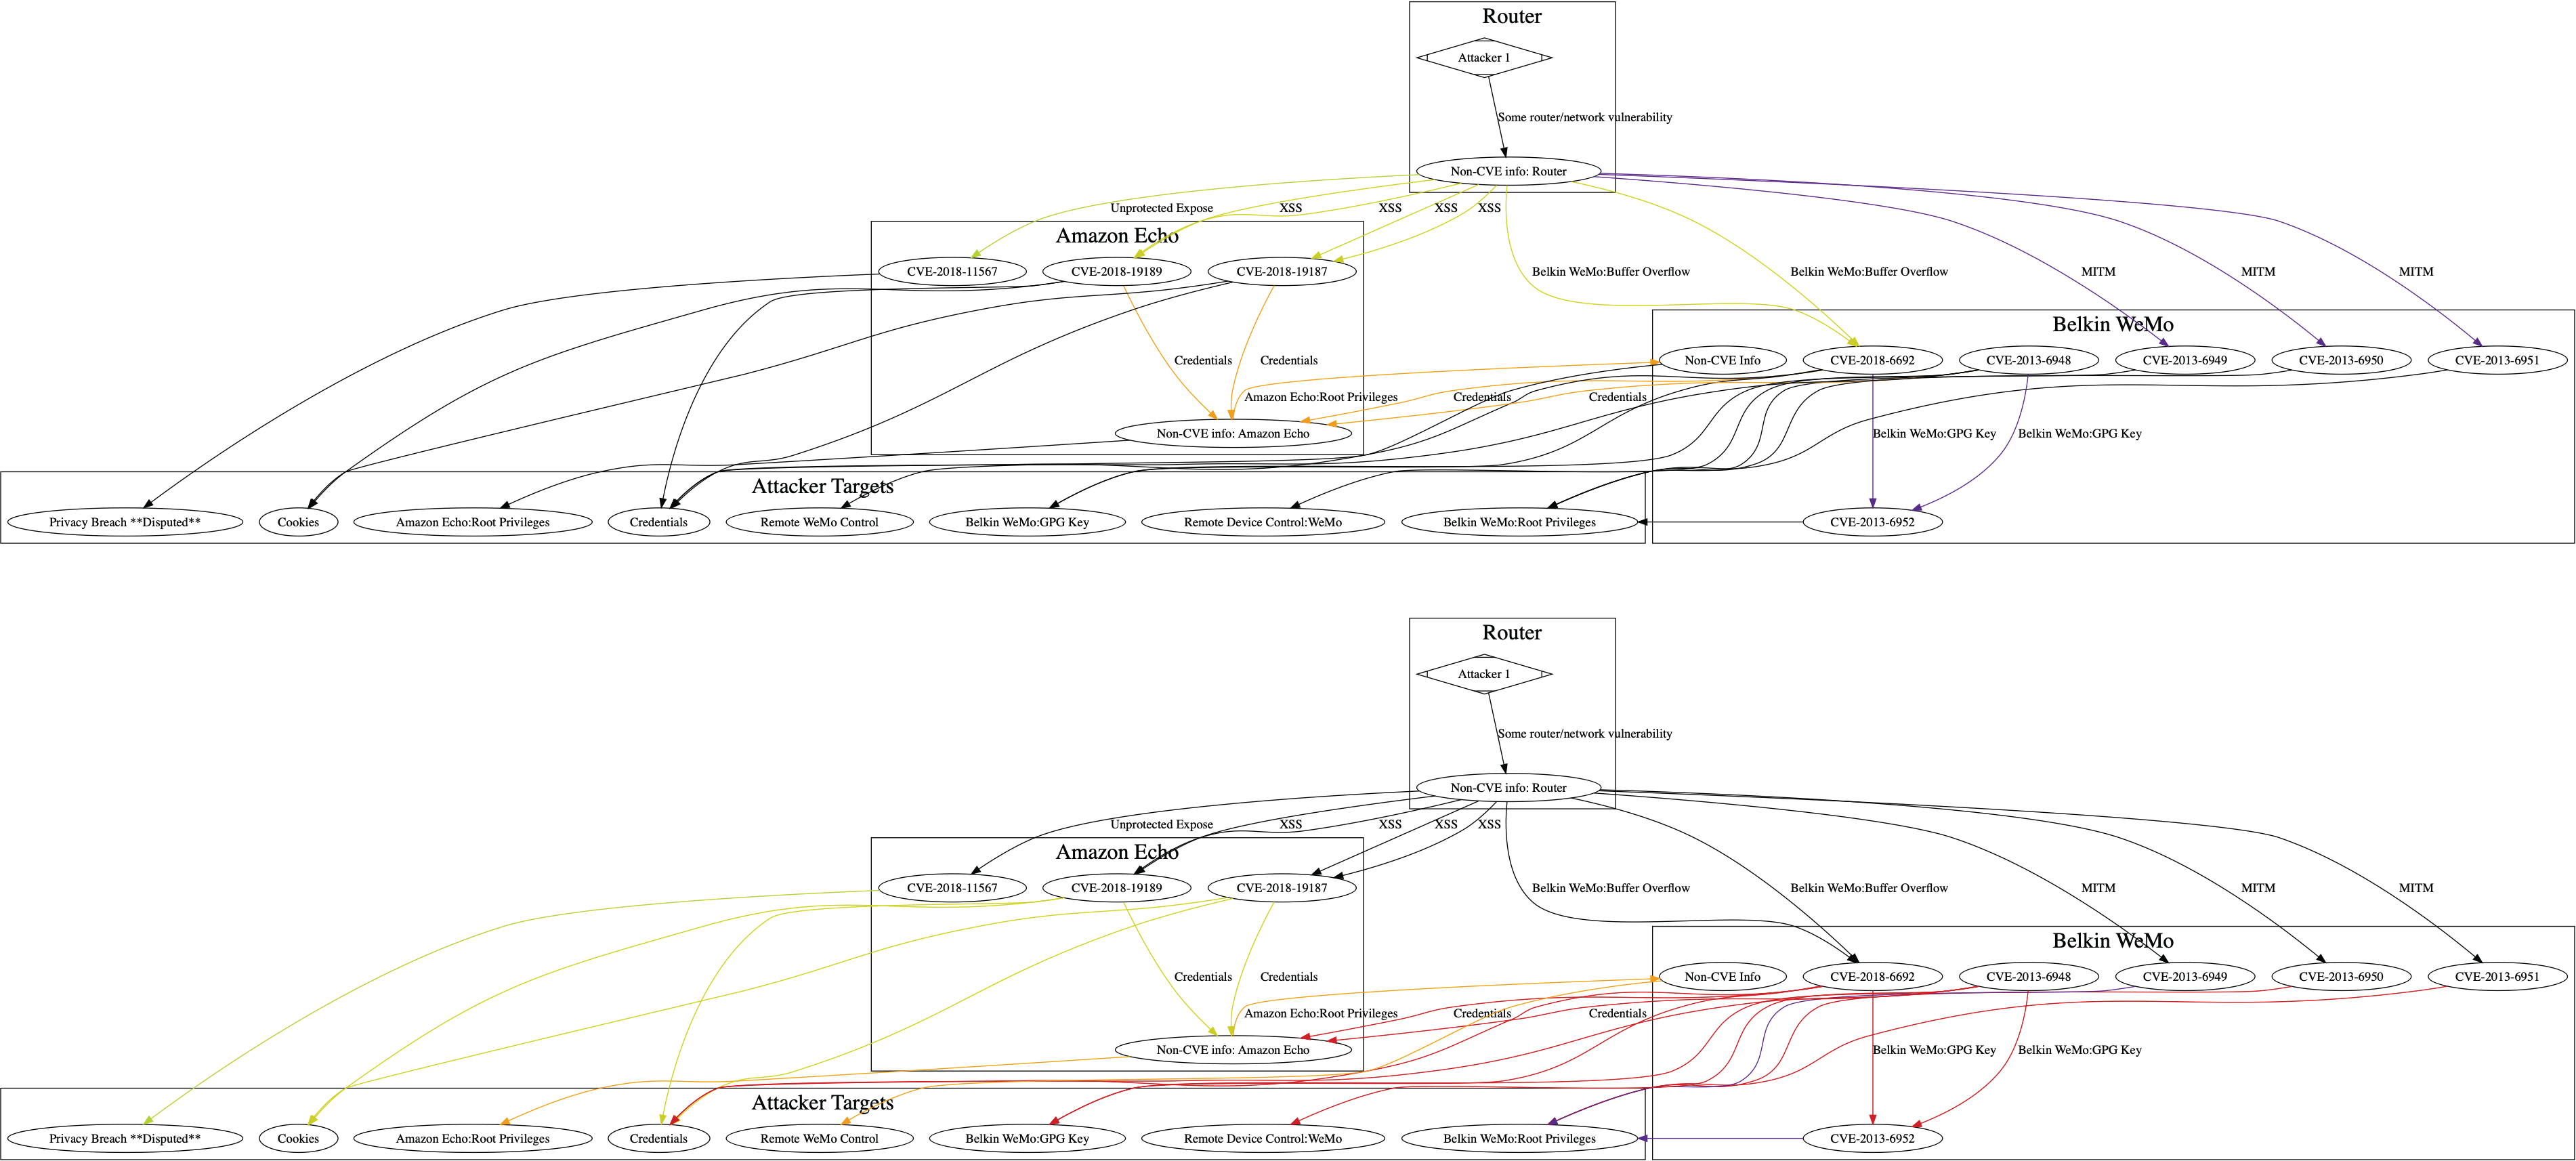
\includegraphics[width=\textwidth]{both2devallcve.png}
    \caption{Exploitability (top) and impact (bottom) circuits corresponding to two devices under the observation of all vulnerabilities. Full-sized images are available in the repository.}
    \label{fig:exp2dev}
\end{figure*}

We evaluate the attack circuit system using a variety of networks and device activity metrics. In our work, we showcase three of these networks: one consisting of one device (an Amazon Echo Dot) with one vulnerability (CVE-2018-11567), one consisting of the Amazon Echo Dot and all of its corresponding CVEs, and one consisting of the Amazon Echo Dot, a Belkin WeMo smart plug, and all of their associated CVEs. The generated exploitability and impact circuits for each of the three settings are shown at the back of this paper in Figures \ref{fig:exp1cve}, \ref{fig:exp1dev}, and \ref{fig:exp2dev}, respectively. Note that the attack circuit complexity grows exponentially with respect to the number of devices in the network, which is visually evident in these figures and is the reason why we primarily focus on smaller networks to demonstrate our work. 

In Table \ref{tab:results}, we record the scores of devices and the network as they were calculated with each of the networks. These results reflect the dynamic activity metrics that we recorded in our experimental observation of the devices over a period of $4$ days, and the output values respond accordingly as we experimentally change the dynamic metrics of the devices (for instance, in contrast to the 1-CVE, 1-device network yielding an exploitability score of $0.0289$ with the Echo's actual status of ``\texttt{rarely\_online}", we noted that the exploitability score rose to $0.0378$ when the device was marked as ``\texttt{frequently\_online}"). Note that where only one device is used, the Belkin WeMo scores are N/A because the device is not present in that network. We select these particular devices to evaluate and illustrate the change in scores when two devices of different levels of vulnerability are added to a network. Based on its three total CVEs, the Amazon Echo's vulnerabilities don't yield as high of a risk, exploitability, or impact score of the device. Its CVEs CVE-2018-11567, CVE-2018-19189, and CVE-2018-19187 have base exploitability scores of $1.8$, $2.8$, and $2.8$, and base impact scores of $1.4$, $2.7$, and $2.7$, respectively. In contrast, three of the Belkin WeMo's six CVEs (CVE-2018-6692, CVE-2013-6952, and CVE-2013-6949) are serious vulnerabilities with base exploitability scores of $3.9$, $10.0$, and $8.6$, and base impact scores of $6.0$, $10.0$, and $10.0$, respectively. Note that in the first column, we observe a network with a vulnerability that is of relatively lesser concern (CVE-2018-11567, with a base exploitability score of $1.8$ and base impact score of $1.4$). When more vulnerabilities are added in, the device's scores all increase as expected, and the network score increases in the same way (because in this setting, the network is defined solely by the device). When the WeMo is added, several paths between the WeMo's vulnerabilities and the Echo's vulnerabilities are discovered from the I/O mapping step, which causes each of the Echo's scores to rise, and the network's scores likewise undergo an increase with the introduction of these new vulnerabilities.

\begin{table}[t]
    \centering
    \begin{tabular}{| c | c | c | c |}
    \toprule
    {} & Echo, 1 CVE & Echo, all CVEs & Echo, WeMo \\
    \midrule
    $E_{Echo}$ & 0.0289 & 0.1182 & 0.3380 \\
    $I_{Echo}$ & 0.0140 & 0.0679 & 0.1776 \\
    Echo $R_{Conf}$ & 0.0073 & 0.0341 & 0.0982 \\
    Echo $R_{Integ}$ & 0.0 & 0.0268 & 0.0910 \\
    Echo $R_{Avail}$ & 0.0 & 0.0 & 0.0644 \\
    \midrule
    $E_{WeMo}$ & N/A & N/A & 0.8490 \\
    $I_{WeMo}$ & N/A & N/A & 0.4823 \\
    WeMo $R_{Conf}$ & N/A & N/A & 0.5744 \\
    WeMo $R_{Integ}$ & N/A & N/A & 0.5649 \\
    WeMo $R_{Avail}$ & N/A & N/A & 0.4605 \\
    \midrule
    $E_{Network}$ & 0.0289 & 0.1182 & 0.9223 \\
    $I_{Network}$ & 0.0140 & 0.0679 & 0.6078 \\
    Network $R_{Conf}$ & 0.0073 & 0.0341 & 0.6367 \\
    Network $R_{Integ}$ & 0.0 & 0.0268 & 0.6239 \\
    Network $R_{Avail}$ & 0.0 & 0.0 & 0.5098 \\
    \bottomrule
    \end{tabular}
    \\
    \caption{Device and network scores for different network settings.}
    \label{tab:results}
\end{table}

\begin{figure}[t]
    \centering
    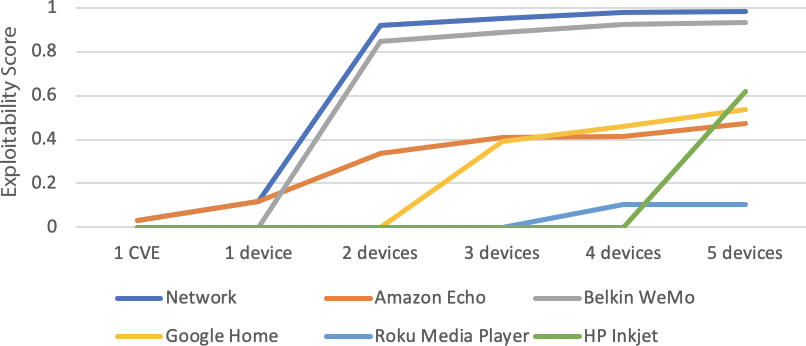
\includegraphics[width=0.45\textwidth]{exploitability_trends.png}
    \caption{Exploitability score adjustment with the addition of new devices (augmented in sequence (left to right, top to bottom)) and CVEs.}
    \label{fig:exploitability_trends}
\end{figure}

This then raises the following question: how can the scores of networks, which are largely heterogeneous and unique, be interpreted relativistically? This is a difficult problem to address, especially without data from real attack circuit use. For now, we normalize the score to a range of $[0,1]$ using a sigmoidal ($\tanh$) function. In general, as the number of devices grows and the vulnerabilities increase, the score trends will demonstrate a sigmoidal behavior, converging to $1$. In Figure \ref{fig:exploitability_trends}, we observe one metric---the exploitability score---of $5$ devices and the overall network, and how it changes as more devices are added. In particular, we start with the Amazon Echo with one vulnerability, then add the rest of the Amazon Echo's vulnerabilities, then add the Belkin WeMo, the Google Home Mini, the Roku media player, and finally the HP Inkjet printer in sequence. As expected, the network's exploitability score approaches a value of $1$ as more devices are added. The case may be made that this scoring method is too sensitive (regardless of the fact that these networks are comprised of devices whose vulnerabilities we know). This may be a result of the dampener and normalization variable values or lack of information about attack circuit behavior in practice. We leave the related refinement of the scoring method to future work.

% Experimental results:

% 1 device (amazon echo), 1 CVE (CVE-2018-19189)
% Echo exploitability:  0.0481128237946 Echo impact:  0.0299910032388 (Echo exploitability:  0.0629167831126 if frequently online)
% Network exploitability:  0.0481128237946 Network impact:  0.0299910032388

% \begin{table}[t]
%     \centering
%     \begin{tabular}{| c | c | c |}
%     \toprule
%     {} & Exploitability Score & Impact Score \\
%     \midrule
%     Echo & 0.0481 & 0.0299 \\
%     Network & 0.0481 & 0.0299 \\
%     \bottomrule
%     \end{tabular}
%     \caption{Device and network exploitability for a network consisting of one device (Amazon Echo) and one CVE item (CVE-2018-19189). Note that if the device is frequently online, the exploitability score changes to $0.0629$.}
%     \label{tab:1cve}
% \end{table}

% 1 device (amazon echo), all CVEs
% Echo exploitability:  0.168507357322 Echo impact:  0.105604770889 (Echo exploitability:  0.21899477347 if frequently online)
% Network exploitability:  0.168507357322 Network impact:  0.105604770889

% Echo exploitability:  0.0288819651753 Echo impact:  0.013999085405 Echo risk confidentiality:  0.0072598724503 Echo risk integrity:  0.0 Echo risk avalilability:  0.0
% Network exploitability:  0.0288819651753 Network impact:  0.013999085405 Network risk confidentiality:  0.0072598724503 Network risk integrity:  0.0 Network risk avalilability:  0.0
% Echo exploitability:  0.118214664357 Echo impact:  0.067895382829 Echo risk confidentiality:  0.0340867888711 Echo risk integrity:  0.0268335568068 Echo risk avalilability:  0.0
% Network exploitability:  0.118214664357 Network impact:  0.067895382829 Network risk confidentiality:  0.0340867888711 Network risk integrity:  0.0268335568068 Network risk avalilability:  0.0
% Echo exploitability:  0.33798508168 Echo impact:  0.177596681443 Echo risk confidentiality:  0.0982420955039 Echo risk integrity:  0.091047160172 Echo risk avalilability:  0.0643708690678
% WeMo exploitability:  0.848966437613 WeMo impact:  0.482286842811 WeMo risk confidentiality:  0.574356582125 WeMo risk integrity:  0.564899552846 WeMo risk avalilability:  0.460542808826
% Network exploitability:  0.922306690621 Network impact:  0.607822022468 Network risk confidentiality:  0.636673729467 Network risk integrity:  0.623860031885 Network risk availability:  0.509800370196

% \begin{table}[t]
%     \centering
%     \begin{tabular}{| c | c | c |}
%     \toprule
%     {} & Exploitability Score & Impact Score \\
%     \midrule
%     Echo & 0.1685 & 0.1056 \\
%     Network & 0.1685 & 0.1056 \\
%     \bottomrule
%     \end{tabular}
%     \caption{Device and network exploitability for a network consisting of one device (Amazon Echo) and all CVE items. Note that if the device is frequently online, the exploitability score changes to $0.2189$.}
%     \label{tab:1dev}
% \end{table}



% 2 devices
% Echo exploitability:  0.187157640205 Echo impact:  0.117455355915
% WeMo exploitability:  0.610551402738 WeMo impact:  0.325690709881
% Network exploitability:  0.715903238257 Network impact:  0.426818500412

% \begin{table}[t]
%     \centering
%     \begin{tabular}{| c | c | c |}
%     \toprule
%     {} & Exploitability Score & Impact Score \\
%     \midrule
%     Echo & 0.1871 & 0.1174 \\
%     WeMo & 0.6105 & 0.3256 \\
%     Network & 0.7159 & 0.4268 \\
%     \bottomrule
%     \end{tabular}
%     \caption{Device and network exploitability for a network consisting of two devices (Amazon Echo, Belkin WeMo) and all CVE items.}
%     \label{tab:2dev}
% \end{table}